\chapter{Object Oriented Programming and Advanced Java Features}
\label{sec:objectoriented}

The biggest step you have to take in mastering Java if you are
coming from the Fortran or C community, is to switch to the object
oriented paradigm. Although C++ programmers are used to objects, there
are quite a number of differences to C++ in Java. That is why Java
xis closer to C than to C++. Since the notions of classes, objects, and
methods are quite abstract we want to introduce them with the help of
a few examples. First we discuss a classical example from probability theory,
the Buffon needle problem using a procedural program and an object oriented version.
A second example will be a class for calculating 
statistical properties of a set of data points stored in a double array.  


%%%%%%%%%%%%%%%%%%%%%%%%%%%
\section{A Classical Example: The Buffon Needle}

It seems that the earliest documented application of stochastic simulation
methods to the solution of an integral has been advanced by Comte de
Buffon \footnote{Georges Loui Leclerc Comte de Buffon ($^*$ Montbard
  (Dijon) 7. 9. 1707, \dag Paris 16. 4. 1788). He was director of the
  Jardin des Plants in Paris and since 1753 member of the Acad\'emie 
fran\c{c}aise. His  work ``Histoire naturelle'', in which theories
about the origin of the earth and of  its organisms aare discussed,
was one of the most famous and translated works of the Age of
Enlightment. Influenced by I. Newton he sustained the scientific
method based on observation and experiment. His work contains many
ideas which entered furure scientific theories.}. The famous Buffon
needle problem has been formulated in 1733 but published only in 1777. It is
supposed
to be the first experiment, a kind of analogue simulation, in the
context of geometric probabilities. The problem can be stated in the
following way: A needle of length $2l$ is drawn at random onto a
horizontal plane ruled with straight parallel lines. The distance
between the lines is $2d (d>l)$. 
What is the probability $P$ that the
needle will intersect one of these lines?

In fact Comte de Buffon performed the experiment of throwing the
needles many times to determine the probability $P$. He also carried
out the mathematical analysis of the problem which we want to review
shortly.

For convenience we denote by $x$ the distance of the middle point of
the needle to the nearest line and by $\phi$ ($0 \le \phi \le \pi$) the
angle between the needle and this line (see
Fig. (\ref{fig:buffondefinition})). The quantities $x$ and $\phi$
completely determine the position of the needle. It is evident from
Fig. (\ref{fig:buffondefinition}) that the needle crosses the line only if
the condition
\begin{equation}
\label{fig:buffoncondition}
x \le l \sin \phi
\end{equation}
is satisfied.

\begin{figure}
\label{fig:buffondefinition}
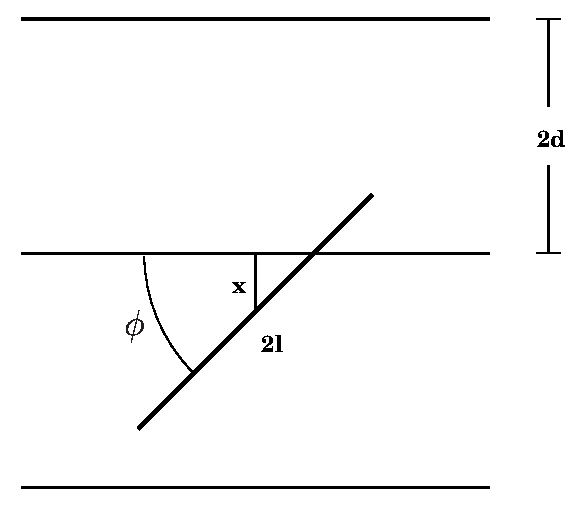
\includegraphics[width=.7\textwidth]{Figures/buffondefinition.eps}
\caption{The Buffon needle problem. Definition of the variables $x$
  and $\phi$.}
\end{figure}

Let us look at the possible positions of the needle in the $x$--$\phi$
plane (see Fig. (\ref{fig:buffonplane})). All positions lying below the
$l\sin \phi$ curve between the abscissa 0 and $\pi$ satisfy the
condition (\ref{fig:buffoncondition}). The surface of this region is
immediately found by integration, $F=2l$. The surface $F$ is a measure
for the set of all positions of the needle which cross one line. On
the other side it is clear that $\pi d$ is am measure for the surface
of all possible positions of the half needle. The ratio of the two
measures $ 2l/\pi d$ is the probability we were looking for, i.e.,
\begin{equation}
\label{buffonprobability}
P = \frac{2 l}{\pi d}.
\end{equation}

\begin{figure}
\label{fig:buffonplane}
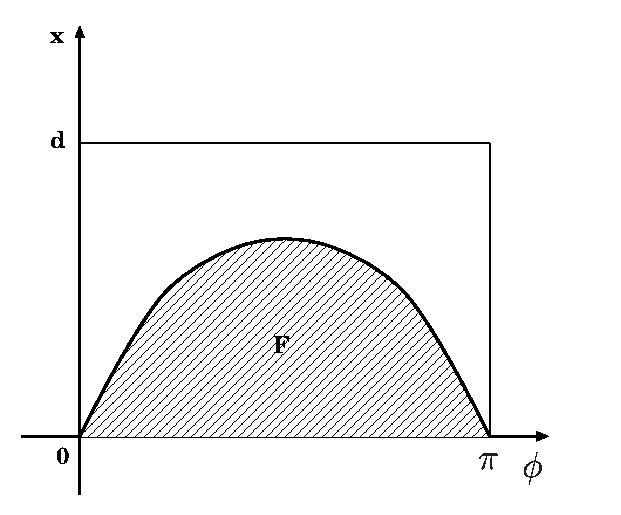
\includegraphics[width=.8\textwidth]{Figures/buffonplane.eps}
\caption{The Buffon needle problem. The $x$--$\phi$ plane (schematically).}
\end{figure}

Some years later (???) Laplace 
\footnote{Pierre Simon Marquis de Laplace, $\ast$ Beaumont--en--Auge
  28.3.1749 \dag 5.3.1827 Paris. Laplace was one of the leading french
  mathematicians of his time. Before being a member in the Acad\'emie
  des sciences and a Professor at the \'Ecole Normale in Paris (1794)
he was an examinator at the \'Ecole militaire in Paris, where in 1785
he examined Naplo\'eon Bonaparte. The most important contributions of
Laplace where in celestial mechanics, cosmology, mathematical physics
and, probability theory. In his work ``Th\'eotie analytique des
probabilit\'es'' (1812) he develops  for the first time a systematic
mathematical treatment of probabilistic problems.} recognized that
the idea behind the Buffon needle experiment could be used to evaluate
$\pi$ from the throws of the needles. Today we would call this a
Monte Carlo determination of $\pi$. If we repeat the experiment $N$
times and count the number of times the needle crosses a line $M$, the
probability $P$ can be estimated by the relative frequency of hits
\begin{equation}
\label{buffonestimateP}
P \approx M/N
\end{equation}
and hence we have with Eq. (\ref{buffonprobability})
\begin{equation}
\pi \approx \frac{2lN}{dM}
\end{equation}
Now, let us try to write a Java code for the simulation of the Buffon
needle problem.

\section{The Traditional (Procedural) Approach}
The traditional approach is straightforward. You just
draw \verb|N| needles and check for each one if it crosses a
line or not. So there are two subroutines. One creates a new
needle with all four coordinates. And the second one is a 
routine, which just compares the lines with the needle coordinates,
whether it crosses the lines or not. You then count the number
of crossings and you get the final estimate of $\pi$.
\inputlisting{Listings_Java/BuffonProcedural.java}

First of all we have made use of the \verb|Math.random()| method, which
draws a random number (a double) between 0 and 1. We also used arrays
to store the coordinates and even used arrays as parameters to
subroutines (methods). The program basically consists of one loop,
which first creates a needle and then checks if the needle crosses
one of the lines in the plane. The first part is done in the method
\verb|drawNeedle()| and creates at random the positions of the start 
and endpoint of the needle. These four coordinates are returned and
stored in the array \verb|needlePos|. The method \verb|checkNeedle()|
uses the positions as arguments and checks if one of the lines is
crossed by the needle, defined by the supplied coordinates.
The variable \verb|cross| counts the number of crossings, which
have occured so far. After the loop has finished we print the
results on the screen.

\section{The Object Oriented Approach - Classes and Objects}
\label{sec:Classes_and_Objects}
Before we begin to write the object oriented code 
we have to introduce some formal aspects of the Java language.

\subsection{Definition of Objects}
We have already met a lot of object oriented features 
without discussing them in detail.  For example, we already noticed
that the fundamental unit of programming in Java is the {\em class}. A
concise definition of classes and objects in Java could be:
\begin{quote}
A class is a collection of data and methods that operate on that data. In
Fortran or C we call the methods procedures or functions. An object
is an instance of the class, meaning it is a thing to work with. The class
defines the data necessary for the object and the functions which can
operate on them.   
\end{quote}

In other words, like in other languages you can compute only with
primitive types (integer, float, ...) but you can also create and
manipulate objects. An example already familiar to us, is the  array. 
If you have an array 
object you can call the method \verb|length| to get the number of
elements of the array. 

So what is the difference to the standard function approach here?
Instead of using function arguments you supply the argument by 
putting them in front of the method separated by a point, e.g., 
\verb|args.length|. The missing brackets on the \verb|length| method
is not a miss-print, the Java engineers thought it might ease writing
array code, but actually it confuses sometimes. Still it is the
most easy demonstration of calling a method of a class.

To calculate the mean of an array of doubles, you can
either write a method which takes the array as an argument (like you would
in Fortran or C) or you can use the object
oriented feature:
\begin{small}
\begin{verbatim}
        import VisualNumerics.math.*;

        double[] array = new double[100]; 
        for (int i=0; i<100; i++) { // create a random array
            array[i]=Math.random(); }
        double result;
\end{verbatim}

\noindent \begin{minipage}{.53\textwidth}
\textbf{Functions}
\begin{sverbatim}
  
 result=Statistics.average(array); 
\end{sverbatim}
\end{minipage}
\begin{minipage}{.41\textwidth}
\textbf{Object Oriented}
\begin{sverbatim}
 Data dat = new Data(array); 
 result = dat.average();
\end{sverbatim}
\end{minipage}
\end{small}
\vspace{.2cm}

The program for the the functional approach is contained in the JNL
package and can be used directly. But the second approach needs a 
new class to be defined by ourself. So here is the code to get the 
second example working. Store this in a seperate file in the same 
directory and compile it before compiling the code above.
\inputlisting{Listings_Java/Data.java}

Which version you prefer seems to be a matter of taste. 
But because all programs in Java are
actually classes we have to understand at least the 
fundamentals of object oriented programming. 
Later on we will have learned the beauty and clarity of the object
oriented approach and the question will turn into: Why do we need
the procedural approach?

Just to remind you again, strings are objects and not primitive 
types. To use strings you first have to declare and instantiate a string
object. Here are three possible ways of doing it:
\begin{sverbatim}
        String text;
        text = "Test String";
        text = new String();
        text = new String("Test String");
\end{sverbatim}
The first line only declares a string object called text and does not
allocate (instantiate) the memory for the value of the object, just
the reference to the value. The second line instantiates and 
defines the String object \verb|text|. The third line instantiates, but
does not define it and the fourth line is like the second line, with
the second line being more efficient in memory consumption and
speed.

An important example of calling methods of classes or objects is
the \verb|.length()| method of the \verb|String| class. In contrast
to the \verb|length| method for the arrays, we have to write the
brackets this time. For example the length of a string can
be printed by using
\begin{sverbatim}
   String s = "text test";
   System.out.println("The length is:"+s.length());
\end{sverbatim}
And if you want to convert the letters of a string to lower case,
you can use the \verb|toLowerCase()| method, e.g.
\begin{sverbatim}
   String s = "TEST Text";
   System.out.println("in lower case letters :"+s.toLowerCase());
\end{sverbatim}


\subsection{The Code of the Object Oriented Approach}
Now we want to
write a Java code which allows the simulation of the Buffon needle
problem. It is clear that in the problem at hand ``needles'' will play
a central role. Each needle may be described by the $x$-- and
$y$--coordinates of  its two ends. Of course, for each needle we can
check whether it crosses a line or not. We draw needles at random so
different needles will have different coordinates. However, needles
have also generic properties which justify to define needles as a class!

The listing of the \verb|Needle| class can be seen below. We are going
to explain basic concepts while discussing this example.
\lstinputlisting{Listings_Java/Needle.java}
The main structure is as follows: The first lines define the 
variables and constants, which a needle should have, like the
length and the position of the needle. These are both properties of
each individual needle contrary to the table dimensions. These are 
still properties of the problem, but they belong to a whole set of 
needles, not only to one. This is visible in the \verb|static| modifier
used in front of the variable definition. So we could actually define
more than one table each consisting of many needles and having different
table dimensions, let us call them planes.

The next part is the constuctor of the class. The constructor is
the code, which gets called if a new object of this class is created with
the \verb|new| keyword. Here you call the constructor by using
\verb|Needle draw = new Needle();| and the constructor just creates
a new needle for this collection of needles belonging to this plane. 

The third part is a method, which returns a boolean variable,
telling us if the needle we are just using is crossing a line of the plane
or not. The difference to the procedural approach enters here: 
How does the method know, which needle to check? This is coded into
the calling program, which takes an object of the needle class
and let the method \verb|crossInspection()| operate on this object. Because
the object consists of all the information necessary for the method,
all the data necessary is already supplied.

Now we are going to talk about these topics in greater detail and try 
to structure all the ideas we have just encountered.


\subsection{Class variables, Constants and Modifiers}
\index{class variables}
\index{constants}
\index{modifiers}
The needle class has four fields which correspond to the four
coordinates which specify the position of the needle. 
The term fields is used in Java as a synonym for variables.
These are the variables different for each needle.

Furthermore, we
need some specification for the geometry involved in the problem.
They are of course not specific to the individual needle, but for
all the needles of a given setup or table. To tell Java that these
variables are for all needles in this setup, you supply the
\verb|static| keyword. The \verb|static| modifier 
defines a field (variable), which is belonging
to the class and not to the object. So every object of that class 
has the same value for a \verb|static| field. 

\index{public modifier}
The \verb|public| modifier
on the other hand defines a field or method, which is special to 
an object not to the class -- this is also called an instance field or
method, the \verb|static| version is called a class variable or
method.

\index{final keyword}
Some of the fields are
defined with the \verb|final| keyword. This is the equivalent to the
const keyword in C. Here the variables with the final keyword are
not allowed to change anymore, e.g. the table dimensions. 

\begin{small}
There is a nice feature to be used with the final keyword. You can
define a final variable, actually computed in an arbitrary method. 
The method is then executed before any other code of the program,
even before the main method. An example would be:
 \end{small}
\lstinputlisting[first=12,basicstyle=\footnotesize]{Listings_Java/TestFinal.java}


\index{modifiers}
\index{variable modifiers}
In Table \ref{tab:modifiers} we give an overview of some available modifiers.
\begin{table}[htbp]
  \begin{center}
    \leavevmode
    \begin{tabular}{l|p{8cm}}
     Modifiers &                                 \\ \hline \hline
     final & variables may not be changed, methods can not be overwritten,
             classes may not be subclassed\\\hline
     public & accessible from anywhere\\ \hline
     static & defines a top-level class, a class variable (field) or 
                 a class method\\\hline
     private & only within the defining class visible, not in other 
               packages, even if subclass of this class\\\hline
     protected & accessible within the package in which it is defined and
                 within subclasses\\\hline
     (none) & accessible only in its package\\
    \end{tabular}
    \caption{Overview of some available modifiers in Java, see also Figure
      \ref{fig:ModifiersGraphics}. For a complete
      overview take a look at page 230-234 in \cite{javanutshell}.}
    \label{tab:modifiers}
  \end{center}
\end{table}
A graphical representation of the access control of variables and
objects is in Figure \ref{fig:ModifiersGraphics}.
\begin{figure}[htbp]
  \begin{center}
    \includegraphics[width=.7\textwidth]{Figures/ModifiersGraphics.eps}
    \caption{A graphical overview of the access 
      control of variables and objects/classes in Java.}
    \label{fig:ModifiersGraphics}
  \end{center}
\end{figure}

It is important to remark that
class variables and methods are the closest relatives to global 
variables in all the other languages. They are accessible from all
classes, but still are belonging to a class. So you could have two
class methods with the same name, but for different classes.

Having fixed also some constants, e.g. $\pi$ and the distance between
parallel lines, we have to initialize the class. This is done by means
of the constructor.

\subsection{The Constructor}
An important part of any class is the constructor of the class. This is
the method (function), which is called when an object of this
class is instantiated. It always has the same name as the class itself.
The constructor can have zero or more arguments and you can even
have different constructors depending on the parameters provided by
the calling syntax.

The constructor of a class ALWAYS calls the constructor of its
superclass, so it is good practice to write \verb|super();| at the
beginning of a constructor to indicate this feature. Because the 
constructor of the super class also calls the constructor of its super
class again, this is called ``Constructor Chaining''.

In our example a needle is initialized in the following way. We draw
at random the four coordinates \verb|needleX1|, \verb|needleX2|,
\verb|needleY1|, and \verb|needleY2| which determine the position of
the first needle. Note, that we have made use of the keyword
\verb|this|.
This keyword is always required when the argument of a method
or a local variable in a method have the same name as one of the fields
in the class. If the method is simple, as it is the case here, it is
not necessary to be that careful.

Here in our example, the constructor just sets the four coordinates
and does not need any parameters to instantiate the needle.

\subsection{Methods and Class Methods}
Having initialized the class we now want to define some methods in our
\verb|Needle| class. There is only one method in our class, which
is the \verb|crossinspection()| method.
The return type of methods always has to be specified, if
there is no return value you have to use the \verb|void| statement
(as in C). The value to be returned is specified by the return keyword.

The method \verb|crossInspection| checks whether
a needle crosses a line or not. The \verb|crossInspection| method
returns a boolean telling you, if the needle crosses a line or not.
Note that the variable \verb|cross| has
been defined as a class variable with the help of the modifier \verb|static|
and gets incremented every time you check a needle, which crosses a line.
With this method our \verb|Needle| class is complete.

Next we need to look at the class \verb|Buffon.java| which contains the
\verb|main| method and demonstrates how to use the \verb|Needle| class,
which is our first example of object oriented coding.
\inputlisting{Listings_Java/Buffon.java}

By defining the \verb|Needle| class in Java, we have created a new
data type. Variables of this type can be declared by
\begin{verbatim}
Needle draw;
\end{verbatim}
\verb|draw| is simply a name that refers to a \verb|Needle|
object (references the object). 
Creating dynamically an object
is done with the help of the \verb|new| keyword
\begin{verbatim}
draw = new Needle();
\end{verbatim}
Next, in a \verb|for| loop we draw \verb|N|  needles and with the help
of the \verb|crossInspection| method we check whether the needles
cross the lines or not and the class variable \verb|cross| is set
accordingly. Finally, the result, i.e. the estimated value
for $\pi$ is printed.



%%%%%%%%%%%%%%%%%%%%%%%%%%%%
\section{Another Example: Calculating the Mean}
Another example demonstrates how to create a class for calculating
the mean of a data set. The mean of a data set $x_i, i=1,\ldots,N$ 
is of course defined as
$$ \text{mean}\quad  <x> \equiv \bar{x} := \frac{1}{N}\sum_{i=1}^{N} x_i.$$ 
The mean is also called the first moment as we will see later and
there are higher moments. They are defined analogously
as
$$ \text{n-th moment}\quad <x^n> :=  \frac{1}{N}\sum_{i=1}^{N} x_i^n.$$  
 
We want to show the
different approaches of programming models in Java. 
You have basically three choices, which are now presented.

\subsection{``Program in One File'' Approach}
First we define variables to set the moments we want to compute.
Then we instantiate and create the data array as an array of
random numbers between zero and one. Then after setting all the moments
to zero, wecompute the moments in a nested loop. The last step
is dividing through $N$ and printing the final result on screen.
\lstinputlisting{Listings_Java/Moments_all.java}

\subsection{``Traditional Procedural'' Approach}
Now we take the computation of the moments and put it into
a method. Then we call the method from our main program. 
Because there is not much difference between the program before
and this one, we just present the differences.
\lstinputlisting[first=20,last=25]{Listings_Java/Moments_procedural.java}
\lstinputlisting[first=32,last=39]{Listings_Java/Moments_procedural.java}


\subsection{Object Oriented Approach}
There are two programs: The first class is
the main program using our own class. This has to be called.
The second one is the
code for the data class itself and have to be compiled only. You can
not start this class. 

We have written two different 
versions to express the difference between a class method and 
an object method.
\lstinputlisting{Listings_Java/MomentsData.java}
The class \verb|MomentsData| includes some new code. First
we use two constructors, whic have different arguments and can
therefore be distinguished by Java. Depending on the calling
syntax using the \verb|new| keyword, you call the first or the second
constructor. 

Then there are two methods defined. Like with the constructor, they
have the same name, but can be distinguished by its argument list.
This is called method overloading in Java. So again depending on
the calling syntax, you call the first or the second method.

Now we take a look at the main program, which uses the above classes.
\lstinputlisting{Listings_Java/Moments_object.java}
Up to line 21 there is nothing new, we just instantiate and create
the data array. Then from line 22 to line 38 the first version using
instance methods is used. The second version from line 40 to line 50
is using a class method. But both versions do exactly the same.
The only difference is line 24 together with line 30 compared to 
line 44 in the second version.
 


%%%%%%%%%%%%%%%%%
\section{Interfaces and Abstract Classes}
Abstract classes/methods 
are also special classes, which can not be instantiated
and contain no code for the (abstract) methods. If you define
some methods, which contain no code as abstract, you have to 
define the whole class as abstract. You can subclass from an 
abstract class and override the abstract methods. You do not have
to override all abstract methods, but then the subclass is abstract
too.

An even more important concept in Java is the interface.
An interface is basically a (abstract) class, which does not implement 
all the
methods defined in the class. All methods have automatically the public
modifier and are abstract.
Therefore you can create classes defining abstract methods,
which should be implemented somewhere else, maybe system dependent, e.g. if you use
the native modifier. Interfaces can be subclassed
to create new interfaces.

Most of the GUI classes of the AWT introduced later are
actually interfaces or abstract classes and not just ordinary classes.
Very useful is this concept for passing methods as arguments to
other methods (see section \ref{sec:PassingArguments}).


%%%%%%%%%%%%%%%%%%
\section{Extending (Inheritance) and Overloading (Overriding) Classes}
Often you want to define subclasses, which should inherit all
the methods and fields from another class. This is easily done
in Java by extending a given class. The meaning of sub-classing is the
notion of data hiding or encapsulation. For example you can write
a subclass, which can not access all the variables of the super class,
therefore hiding some details. 

You can reference the super (parent) class by applying the
\verb|super| modifier in front of a method or variable of
the parent class. And the \verb|this| modifier always refers to
the actual class. 

You can also have equal names for a variable in the super class and the
child class, which means you have to reference the variables explicitly
by using the \verb|super| or \verb|this| keywords. If you want to refer
to a variable two classes up from the actual class, you have to use
the notion of ``shadowing'' \cite[]{javanutshell}, which is a kind of
casting with classes. 

If you define a class to be final, it can not be extended.
For example the java.lang.System class is a final class.

Different from C++,  you can not inherit from more than one class
in Java, meaning that there is always only one superclass for each
class. 
The only way of having multiple inheritance is by using
interfaces, which we will not cover extensively in our introduction.

If you write a subclass you can overwrite methods already defined
in the super class. This is called overloading of methods,
analogous to the C++ overloading. But in C++ you can even
overload operators like +, -, etc., which is not possible (in Java 1.1) yet.

A simple example is given by the
HelloWorld\_Applet.java program in section \ref{sec:Applet}.
There we have extended the Applet class of the Java.applet package
and therefore making our program a subclass of the Applet class.
So we inherited all the methods and fields of that class. Then we
overloaded the \verb|paint()| method to display our message. 
In the words of object oriented programming, writing an applet is
called: defining a subclass of the Applet class and overloading
the methods of the Applet class as necessary.

One nice and important feature in Java is, that all classes which
do not have an explicit parent, inherit from the \verb|java.lang.Object| 
class. So you can call this class the father of all classes.
There are only a few methods defined in this (abstract) class,
which you can always override. For example the \verb|toString()| 
method is in \verb|java.lang.Object|. If you override this method,
you can define your own objects, which can then be printed by
the usual \verb|println()| commands. 

As an example let us write a simple class, which 

In Table \ref{tab:JavaLangObject}
all methods defined in \verb|java.lang.Object| are displayed.
\begin{table}[htbp]
  \begin{center}
\begin{small}
\begin{verbatim}
public boolean equals (Object obj);
protected Object clone() throws 
               CloneNotSupportedException, OutOfMemoryError;
public String toString ();
public int hashCode(); 
protected void finalize() throws Throwable;
\end{verbatim}
\end{small}
    \caption{All methods belonging to the (abstract) 
               \texttt{java.lang.Object} class.}
    \label{tab:JavaLangObject}
  \end{center}
\end{table}

If you want to find out about all methods and fields available
in the \verb|java.lang.object| class in detail, you just take
a look at the Java API docuementation of the JDK. There in the
package API documentation  you
click on the package \verb|java.lang| and then on the class
\verb|object| and you get the full description of the class
with all methods and fields.


%%%%%%%%%%%%%%%%%%%%%%%%%%%%%%%%%%%%%%%
\section{The System Class: Screen-Output and Keyboard-Input}

Now we are in a place to discuss the \verb|System.out.println()| statement
already used in the ``HelloWorld'' program. This is calling the
\verb|println()| method of the \verb|PrintStream| class of the java.io 
package. And the \verb|out| is a variable from the System 
class of the java.lang package, referencing the \verb|PrintStream| class. 

There are also two more variables called \verb|err| and
\verb|in| for error output and data input. 
The java.lang.System class in general provides an platform-independent 
interface to some system functions.

Here an example demonstrating some of the material we have learned and
explains how to get any kind of input from the keyboard.
It waits for an user input and just echoes the typed characters
until you type the word ``Java''. 
\inputlisting{Listings_Java/System_Class.java}

Let us analyze the program:
First look at line 19, where we have used the \verb|print()| method
of the System class. It does the same as \verb|println()|, but does not
jump to the next line after the output.

Then take a look at line 23, where we compare two strings. 
We have to use the \verb|equals()| method of the String class to
compare the value of two strings and not the references. 
In line 25 we use the string concatenation operator $+$ for the output.

By the way, you have probably already noticed, that 
the \verb|for(;;)| loop in line 17 is a endless loop.

The actual input takes place in line 21, where we assign the input
to the string \verb|line|. The method used is \verb|readLine()|, which
is a method of the \verb|BufferedReader| class. It reads input until
a carriage return is reached. The actual object of the 
\verb|BufferedReader| class is created in line 13. To that end we have
to create a Reader class for the \verb|InputStream| called \verb|in|
just mentioned above (this is done in line 11).

Because we are using I/O commands, we have to take care of exceptions
which can occur during the I/O. For that reason we have to use the
\verb|throws IOException| statement in the definition of the main
class (see line 7).

A last remark concerns the escape codes used in line 15 and line 25.
The first one, $/$'' displays a quotation mark and the second
one a newline.
To include arbitrary formatting (escape) characters
to the string supplied to the print() and println() methods, you
can use similar to C the \verb|\n|, \verb|\t| or \verb|\\| codes
to get a newline, a tab or a backslash in the output. You should 
also note that, if you use e.g. \verb|System.out.println(5+7)| you
get \verb|12| as output, so if you want to see \verb|5 7| you have
to use 
\begin{sverbatim}
|System.out.print(5+" "+7)
\end{sverbatim}

Although this looks very complicated, if we do not want to go into
details, just copy this part to a program and reuse the code.
But after we get used to object oriented programming we will not have
any problems understanding the code above anymore.

\subsection{Easy Input and Lava Rocks printf()}
\label{sec:LavaRocks}
Another easy solution is to use the \verb|EasyIn| and the
\verb|Printf()| methods, supplied by our \verb|simulation| class
and the ''Lava Rocks''\footnote{This is a freely available package,
containing some easy to use methods, mostly for C programmers
who switched to Java. For details see \cite{LavaRocks}.} package.

\paragraph{Easy Input}
You can easily use these methods to get input from keyboard
for different primitive data types. For example to input
a primitive data types, you just use
\begin{small}
\begin{verbatim}
import simulation.*;
 .....
 double  d = EasyIn.readDouble();    // reads double from System.in
 int     i = EasyIn.readInt();       // reads int from System.in
 float   f = EasyIn.readFloat();     // reads float from System.in
 boolean b = EasyIn.readBoolean();   // reads boolean from System.in
 .....
\end{verbatim}
\end{small}

\paragraph{Lava Rocks -- printf()/sprintf()/fprintf()}
To use the Lava Rocks package you could write a code like
\begin{small}
\begin{verbatim}
 import lava.clib.*;
 .....
 int i=100;
 float f=165.234f;
 Stdio.printf ( "%8d and %8.1f : test text\n", new Object [] { 
                             new Integer(i), new Float (f) } );
 .....                 
\end{verbatim}
\end{small}
Remember that you need the \verb|lava.jar| file in the classpath.
The output will look like
\begin{verbatim}
     100 and    165.2 : test text
\end{verbatim}
If you are familiar with the C routines, then you can find all
the modifiers used for formatting the different types of variables
in Table \ref{tab:PrintfModifiers}.
\begin{table}[htbp]
  \begin{center}
    \begin{tabular}{cl}
      Modifier & Type to be formatted \\ \hline
      \%bd & byte \\
      \%hd & short \\
      \%d & signed integer \\
      \%ld & long \\
      \%u & unsigned integer \\
      \%o & unsigned octal integer \\
      \%x / \%X & unsigned hexadecimal integer (lower or uppercase)\\
      \%f & float \\
      \%lf & double \\
      \%e / \%E & float, scientific notation \\
      \%g / \%G & float, same as f or e, depending on value \\
      \%s & String \\
      \%c & character\\
      \%p & object identity hash code in unsigned hexadecimal \\
      \%$\backslash$n & platform independent line seprarator\\
      \%n & counts characters\\
    \end{tabular}
    \caption{All possible modifiers to be used in the format 
      string given to the printf()/sprintf()/fprintf() methods supplied 
      by the Lava Rocks package.}
    \label{tab:PrintfModifiers}
  \end{center}
\end{table}
The modifiers represent the place, where the actual value of the variable 
has to be inserted before the output is sent to the screen (or file, 
or string). So you have to make sure that the order of the modifiers and
the order of the supplied variables is correct, otherwise you get
unpleasant results or strange errors.

There are three additional things to mention: 
If you use the
same format string (the first argument to the printf method) 
very often, you can speed things up by saving the format string
and only use the variable every time, like:
\begin{small}
\begin{verbatim}
   import lava.clib.stdio.*;
   .....
   PrintfFormatString fmt = 
      new PrintfFormatString ("%8d and %8.1f : test text\n");
\end{verbatim}
\end{small}
Now you can use \verb|fmt| instead of the string in all printf commands
and it will be much faster.

There is also an ``easier'' way of using printf without creating
an object array, which is much more inefficient and should be avoided.

And there is a platform neutral code for newlines: Use \verb|%\n| instead
of \verb|\n| in the format strings and you always get a newline,
no matter which platform you run the program.

The same holds for the other two methods \verb|sprintf()|, which writes
the formatted output to a stringbuffer (we will discuss this in section
\ref{sec:FileIO} and in section \ref{sec:Symphony} in more detail.),
and \verb|fprintf()|, which writes the output to a file (actually a
Writer, see section \ref{sec:FileIO}).

There is another free implementation of the printf command for
Java called \verb|Format.java| of the \verb|corejava| package.
But it has much less functionality and so we decided to use
the Lava Rocks implementation.

%%%%%%%%%%%%%%%%%%%%%%%%%%%%%%%%%%%%%%%%%%%%%%%%%%%
\section{Passing Arguments to Methods}
\label{sec:PassingArguments}
We want to review all the aspects concerning the passing of
arguments to methods or -- for former FORTRAN programmers --
passing arguments to subroutines/functions.

\paragraph{Global Variables}
First of all there is of course always the possibility to 
pass variables as global variables. This is easy to use,
but it makes it difficult to follow a program structure.
So it is preferred to use arguments to methods in an
argument list.

\paragraph{Primitive Data Types}
The important point to note here is that Java always
passes primitive data types by value and all the other
arguments by reference (reference data types). 
This means that all primitive
variables of the argument list can be changed within
the method. The dummy variables used in the method 
can be viewed as local variables.

\paragraph{Reference Data Types}
The reference data types (e.g. arrays, objects, etc.)
are passed by reference and therefore only the memory
address is passed to the method. That is again the reason that
by using the standard assignment or comparison operators,
you do not compare the values of the reference data type, but
the memory addresses where the data is stored. Therefore there
is the \verb|equals()| operator used for comparing reference data
types. By the way there is no method
of getting the actual memory address for a reference data type,
which would be a severe security problem.

If you pass a reference data type to a method it should be
clear, that every change of the dummy variable used for
the reference data type used in the method, will result in a change
of the passed reference variable. So for example for arrays:
\begin{lstlisting}{}
  .....
  public void main (String[] args) {
    ...
    int[] array = {1,2,3,4,5};
    test(array);
    ...
  }
  public void test(int[] dummyarray) {
    int length=dummyarray.length;
    for (int j=0; j<length; j++) {
      array[j]=0;
    }
  }
  .....
\end{lstlisting}
In this example we pass an array of integers, where the values are all 
not zero. In the subroutine we change the values of the 
\verb|dummyarray| array.
But we passed only the memory location, so the change is actually
a change in the \verb|array| array. If you print the result after
the call to the method, all elements are zero!

If you now think about changing a primitive data type inside a method 
passed to it, there is none. There is actually 
no simple way of using reference types for primitive data types to
change method parameters. 

\paragraph{Instance Variables}
A nice and clear way of passing arguments between methods, is
using instance variables. The problem here is that you have
to create a new class and define instance variables for it.
Then you can instantiate an object of this new class and
change the values of the instance variables from the main
program or the methods therein. But still you have the problem
of passing the instance to the methods.

\paragraph{Multi-Dimensional Arrays as arguments}
As a scientist you will always have the necessity to use arrays
as arguments to methods. There is actually no trouble with using
for example a 1D array to a method, which expects a 1D array. But 
what if you have a 2D array and the method needs a 1D array as
an argument? Should you copy a 1D row or column of the 2D array
into a new 1D array and then call the method or is there a better
way? 

The answer is yes, but not in all cases. You can always omit 
the last dimensions of an array. For example if you leave out
the second dimension of a 2D array, you get a 1D array, which is 
just the desired row of the array. But there is no way of referencing a
column. The following program demonstrates the usage.
\inputlisting{Listings_Java/testArray.java} 

\paragraph{Methods (Functions) as Arguments} 
Especially for scientists it is of great importance to know how
to pass a function (method) to another method.

The first solution would be to write a method as a class method,
therefore accessible from every instance of the class and
so you do not need to pass the method as an argument at all.

The second solution is much more versatile and general.
But as always you have to do more work. You need an interface,
which defines the function you would like to pass to a method
(Declaration). Then you need a class, which implements this
interface, therefore representing the real function (Implementation).
And at last you write your program/class, which instantiates
the former class and now you can pass the function by reference
to all methods you like (Usage).  

Here a short example:
\paragraph{Declaration} 
\begin{verbatim}
  interface function {
    double f (double x); 
  }
\end{verbatim}

\paragraph{Implementation}
\begin{verbatim}
  class SquareFunc implements function {
    public double f (double x) {
       return (x*x) ;    //  <----- here is the actual function
    }
  }
\end{verbatim}

\paragraph{Usage} 
This is the program, which uses the two classes/interfaces above.
\inputlisting{Listings_Java/TestPassingFunctions.java}

%%%%%%%%%%%%%%%%%%%%%%%%%%%%%%%%
\section{Structure and Overview of Java}

%%%%%%%%%%%%%%%%%%%%%%%%%%%%%%%%%%%%%%%
\subsection{Packages in Java 1.1 and Java 2}

Here we list all the standard packages (APIs) included in the Java 1.1
language standard. The important packages (for our purposes) are
written in small caps.

\subsubsection{Java 1.1 Packages}
\begin{description}
\item[\textsc{java.applet}] includes the superclass of all Java applets (small package)
\item[\textsc{java.awt}] the Abstract Windowing Toolkit (large package)
\item[java.awt.datatransfer] provides data exchange between programs
\item[\textsc{java.awt.event}] event handling for the AWT (Mouse, etc.)
\item[java.awt.image] rarely used classes for image processing (use AWT) 
\item[java.awt.peer] rarely used interfaces for the AWT
\item[java.beans] interfaces and classes for beans programmer
\item[\textsc{java.io}] all the input/output classes (very big)
\item[\textsc{java.lang}]  central Java language classes (largest package)
\item[java.lang.reflect] part of the Java Reflection API (small)
\item[\textsc{java.math}] arbitrary precision arithmetic (small)
\item[java.net] networking package
\item[java.rmi] RMI is Remote Method Invocation. It is a mechanism that enables an object on one Java virtual machine to invoke methods on an object in another Java virtual machine. 
\item[java.rmi.dgc] RMI distributed garbage-collection (DGC). 
\item[java.rmi.registry] Methods to access the RMI registry.
\item[java.rmi.server] RMI server classes and methods.
\item[java.security] A security framework. This includes classes that implement an easily configurable, fine-grained access control security architecture.
\item[java.security.acl / java.security.cert / java.security.interfaces / java.security.spec] Additional security features.
\item[java.sql] Provides the JDBC (Java Database Connectivity) package. JDBC is a standard API for executing SQL statements.
\item[java.text] for writing internationalized programs (date, time, etc.)
\item[\textsc{java.util}] useful classes, often used, e.g. millisecond time,
  calendar, random numbers, vectors, etc.
\item[java.util.zip] data compression and decompression classes
\end{description}

\subsubsection{Java 2 Packages}
Additional API packages in Java 2 are:
\begin{description}
\item[java.awt.color] Provides classes for color spaces.
\item[java.awt.dnd] Provides interfaces and classes for supporting drag-and-drop operations.
\item[java.awt.font] Provides classes and interface relating to fonts. It contains support for representing Type 1, Type 1 Multiple Master fonts,
OpenType fonts, and TrueType fonts. 
\item[java.awt.geom] The Java 2D classes for defining and performing operations on objects related to two-dimensional geometry. 
\item[java.awt.im] Classes and an interface for the input method framework. This framework enables all text editing components to receive Japanese, Chinese, or Korean text input through input methods. 
\item[java.awt.image.renderable] Classes and interfaces for producing rendering-independent images.
\item[\textsc{java.awt.print}] A general printing API, including document types, 
  page setup and formats and job control dialogs.
\item[java.beancontext] A bean context is a container for beans and defines the execution environment for the beans it contains.
\item[java.lang.ref] Provides reference-object classes, which support a limited degree of interaction with the garbage collector.
\item[java.rmi.activation] Provides support for RMI Object Activation.
\item[java.util.jar] For reading and writing the JAR (Java ARchive) file format, which is based on the standard ZIP file format with an optional manifest file. 
\item[javax.accessibility] Defines a contract between user-interface components and an assistive technology that provides access to those components. 
\item[\textsc{javax.swing}] Provides a set of "lightweight" (all-Java language) components that, to the maximum degree possible, work the same on all
platforms. 
\item[java.swingx.*] There are 15 more packages in the Swing package, which we are not describing here in detail. Take a look at the Swing tutorial or documentation.
\item[org.omg.CORBA] Provides the mapping of the 
  Object Management Group (OMG) CORBA\footnote{Common Object
    Request Broker Architecture} APIs to the Java programming language, 
  including the class Object Request Broker (ORB), 
  which is implemented so that a programmer can use it as a 
  fully-functional Object Request Broker.
\item[org.omg.*] 6 more packages are provided for using CORBA with Java. 
  See the API documentation.
\end{description}

\subsection{Reserved words in Java}
The following words are reserved for Java and can not be used for names
of classes, variables or methods:
\begin{sverbatim}
abstract, boolean, break, byte, byvalue, case, cast, catch, char,
class, const, continue, default, do, double, else, extends,
false, final, finally, float, for, future, generic, goto, if,
implements, import, inner, instanceof, int, interface, long,
native, new, null, operator, oouter, package, private, protected, 
public, rest, return, short, static, strictfp, super, switch, 
synchronized, this, throw, throws, transient, true, try, var,
void, volatile, while, widefp
\end{sverbatim}

%%%%%%

\section{Name Conventions in Java}
In order to make the Java codes more readable it is customary to stick
to the followinh name conventions.

\paragraph{Classes and Interfaces.} The names of classes and interfaces
  should consist of one or more words which are concatenated. They
  should describe appropriately the class and the interface. 
  The first letter of the name is an uppercase letter. If the
  class name consists of more than one word, each word after the first
  one begins with an uppercase letter, e.g., \verb|Needle|,
  \verb|Reader|, \verb|StringToken|.

\paragraph{Methods.} The names of methods are verbs or verb--phrases. 
  They begin with lowercase letters. If the name consists of
  more than one word, the second and all the following words begin
  with an uppercase letter. To give some examples:
\begin{itemize}
\item methods, which set the value of a variable or return the value of
  a variable begin with \verb|set| or \verb|get|; e.g.,
  \verb|setName|, \verb|getData|.
\item methods, which check some condition and return a result  get the
  prefix \verb|is|, e.g., \verb|isSmaller|.
\item methods, which simply perform some conversions are characteized
  by the returned type and have the prefix \verb|to|, e.g.,
  \verb|toString|.
\end{itemize}
If you stick to these rules you are already writing programs, which
conform to the Java beans syntax. This means you can take your
programs and use them as beans later on with almost no changes
(see section \ref{sec:Beans}).


\paragraph{Instance Variables.} Names for instance variables are
  words, nominal phrases, or short--hand notations. Like names for
  methods the word begins with a lowercase letter and all following
  words begin with an uppercase letter, e.g., \verb|next|,
  \verb|dataVector|,
\verb|minValue|.

\paragraph{Local variables or parameters.} Local variables should get
  short  names. Usually, they are named by sequences of small
  letters. Typical examples are acronyms (the first letter of each
  word) of the name of the class for a variable, which keeps a
  reference to an instanace of the class, e.g., \verb|rv| for Random
  Variable or short--hand notations, e.g., \verb|minx| for the minimal
  value of the variable x. Single letter names should be avoided,
  unless for temporary variables or variables, which are used in
  loops or for variables with an uncertain value of some type:
\verb|b| for \verb|byte|, \verb|c| for \verb|char|, \verb|d| for
  \verb|double|, \verb|e| for Exception, \verb|f| for \verb|float|,
  \verb|i|,
\verb|j|, \verb|k| for \verb|int|, \verb|l| for \verb|long|, \verb|o|
  for \verb|Object|, \verb|s| for \verb|String|.

\paragraph{Constants.} The names of constants may be composed by one
  or more words. All characteres are upper--case letters and the words
  are joined by \verb|_|, e.g., \verb|PI|,  \verb|MIN_VALUE|.

\paragraph{Packages.} Packages, which are only used locally are
  identified by a name which begins with a lower--case letter. This
  word can not be \verb|java|; this keyword is reserved for
  standard Java classes.



\section{Java Documentation}
As the time of writing the JDK (1.1 or 2) is distributed in
a twofold way: The first one is the Java Runtime Environement called JRE,
which includes the Java virtual machine, the Java plugin for 
the Internet Explorer
and Netscape to run Java applets. 
\index{JDK!documentation}
\index{JDK}

The second one is the complete package -- 
the JRE and additionally all development tools to write Java programs.
The API documentation is included in the full package, but not
in the JRE. The documentation for the APIs is also available seperately.

In the directory \verb|JAVA_HOME|, on UNIX this could be 
\verb|/usr/local/jdk1.2|, \verb|/usr/local/lib/jdk1.2| or 
\verb|/usr/lib/jdk1.2| and on Windows this might be \verb|c:\jdk1.2|, 
you can find all the documentation in the subdirectory
\verb|docs|. It is best viewed using a web browser
starting with the page \verb|jdk1.2/docs/index.html| 
(see also Figure \ref{fig:JDKFiles}).
\begin{figure}[htbp]
  \begin{center}
    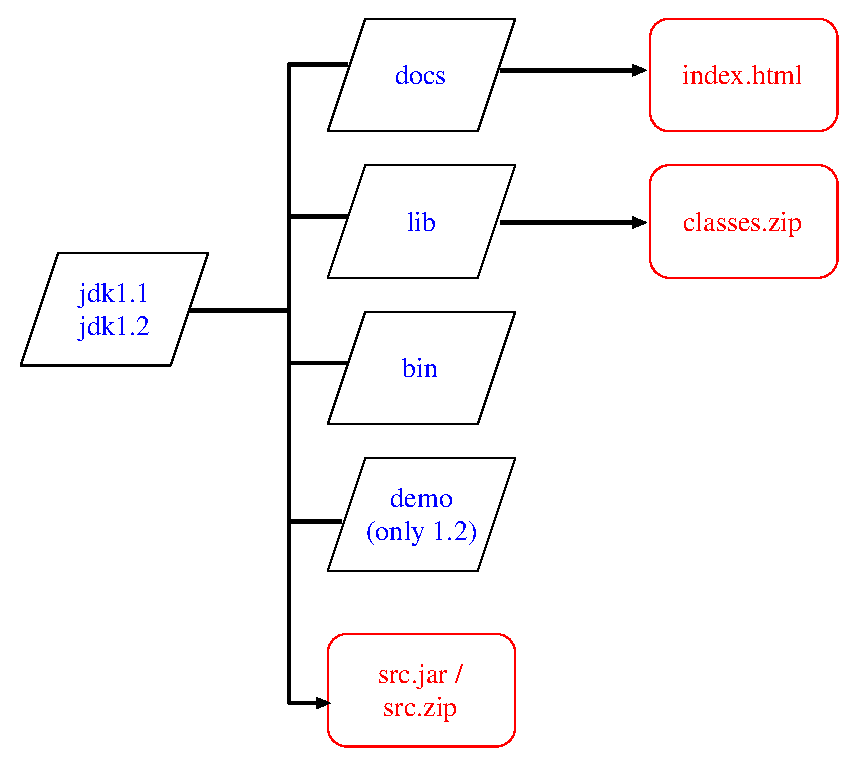
\includegraphics[width=.6\textwidth]{Figures/JDKDocumentation.eps}
    \caption{The file structure of the JDK distribution, 
      both the binary and the documentation package.}
    \label{fig:JDKFiles}
  \end{center}
\end{figure}


%%%%%%%%%%%%%%%%%%%%%%%%%%%%%%%%%%%%%%%%%%%%%%%%%%%%%%%%%%%%%%%%%
\section{Applications and Applets Revisited}

After discussing object oriented programming,
we want to recapitulate the basic differences and features of
the two possible ways of writing and starting Java programs.

\subsection{Applications}
A Java application is in the traditional language a ``normal'' program.
In Java slang it is a class, which only has to have a \verb|main|
method, which has to be \verb|static| and \verb|public|. This is also of course the
entrance point, if you start the Java application. Then the program
executes sequentially the code given in the main method (of course it
goes parallel, if you use threads somewhere in the application - see
\ref{sec:ParallelJava}). There are no restrictions of any sort using
features in an application.


\subsection{Applet}
An applet is a Java class, which can be loaded into a virtual machine
and can then be executed by it. 
For example a web browser could load
the applet, check if it is an applet allowed to be started on the
machine the browser is running on and then ``starts the applet''.

This is basically the most confusing part of an applet: What are the
instructions, which get executed when the browser ``starts the applet''?
To that purpose go ahead and write a simple program 
(see the program \verb|ShowTrace.java| in the appendix \ref{sec:ShowTracePrg}),
 which only 
prints out the place where the execution just takes place and ``start''
the Java class on the command line as an application, in the appletviewer
as an applet and in a browser as an applet. What you will get is shown
in figure \ref{fig:LineOfExecution}.
\begin{figure}[htbp]
  \begin{center}
    \leavevmode
    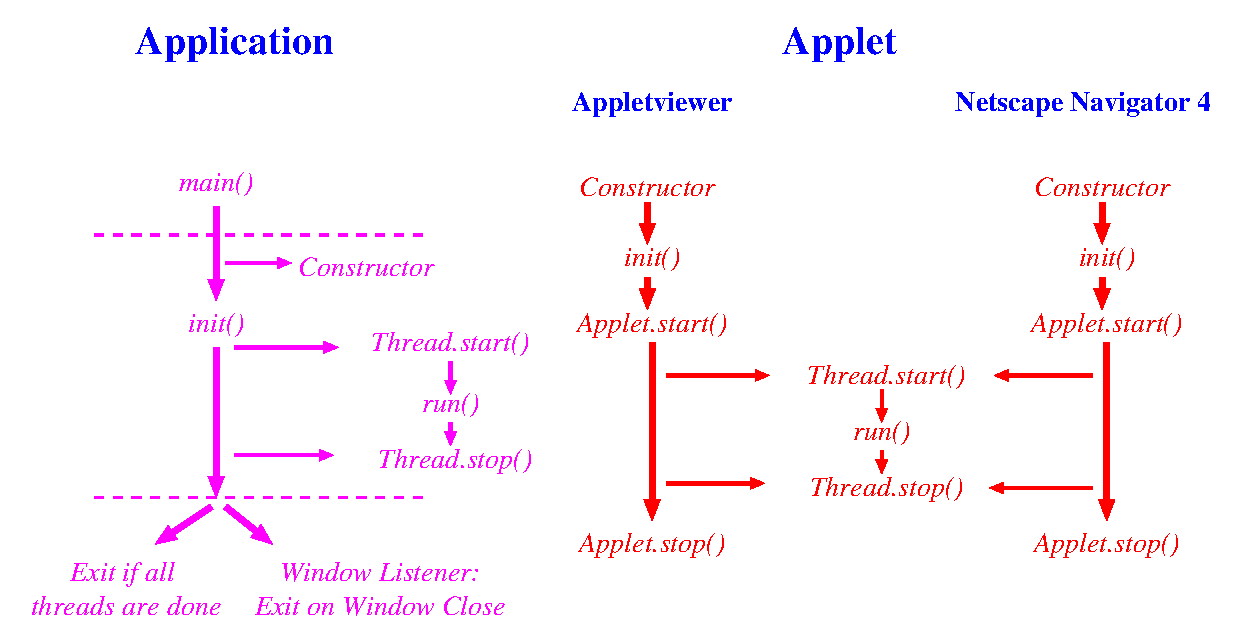
\includegraphics[width=\textwidth]{Figures/LineOfExecution.eps}
    \caption{The line of execution in an application and an applet in
        the appletviewer or the Netscape Navigator 4.08. For the application
        only the part above the first line and below the second line are
        actually the parts, which can not be avoided. The remaining
        part is just provided to show you how to write an application,
        which can be used as an applet, too.}
    \label{fig:LineOfExecution}
  \end{center}
\end{figure}

So for the applets you have to write (implement) at least the 
\verb|init()| method to get things going. But now you will ask, why did we
not supply an  \verb|init()| method when we wrote our first 
HelloWorld applet? The answer is we did, but we did not write it explicitly,
because we left it empty. The trick was that for an applet there is
always another thread (see 
Chapter \ref{sec:ParallelJava} for an introduction to threads)
running, which takes care of (re)painting the windows (panels) used by the applet.
This thread is a method of the AWT package (see Chapter \ref{sec:AWTIntro}) and
the method is the \verb|paint()| method. And in the    HelloWorld applet
we have overriden the \verb|paint()| method to display our message.

Actually the threads and methods used for painting and repainting
the windows or panels is a little bit more tricky and involved, so we
have to postpone the discussion to a later chapter. Here only the basics:
There is a method \verb|repaint()|, which calls the \verb|update()|
method and that in turn calls the \verb|paint()| method, when there is time
to do so. This sounds very complicated in the first place, but 
it will be resolved later on.

There is another issue to be addressed here in the context of applets.
So far we have always written a separate HTML file to use with the
appletviewer, which then in turn calls the applet itself. The burden
of having two files for one applet can be avoided by putting the
HTML Code at the beginning of the Java class file in a comment. Then
if you call the appletviewer with the Java class file 
it executes the HTML code supplied
in the Java class file and starts the applet. It even starts in
the Netscape Navigator, although it probably makes no sense for
large programs embedded in a set of HTML pages kept uptodate in a
different way as the Java source code. But it certainly eases
writing small applets and getting not confused by too many files on
your disks. 

Here a small example showing the described feature:
\inputlisting{Listings_Java/test_Applet.java}
You can start it (first you have to compile it) 
by typing \verb|appletviewer test_applet.java| or 
in the Netscape Navigator type 
\verb|file:/home/user/test_Applet.java|\footnote{You have to substitute 
the path by an appropiate one for your system and configuration.}.
Then on the command line or the terminal with which you started the browser  
you see the short message.


\subsection{Programs as Applets and Applications}

??? GUIs ....

To write a class to be run as an applet and an application
you can see in Figure \ref{fig:LineOfExecution} the correct order
of the methods, which get called in both cases. As an example, 
we have used the following template for the 
bigger programs
to have them run as an applet as well as a standalone application.
We have to add code to the \verb|run()| and the \verb|Setup()| methods
to get a useful program. The  \verb|Setup()| method should contain all
screen setup or preliminary work. In the  \verb|run()| method goes
the computational intensive part of the program.
\inputlisting{Listings_Java/TestAppletApplication.java}


%%%%%%%%%%%%%%%%%%%%%%%%%%%%%%%%%%%%%%%%%%%%%%%%%%%%%%
\section{Higher Mathematics in Java}

\subsection{Standard Mathematical Functions in Java}
\label{sec:Standard_Math}

The standard mathematical functions of Java are declared in the 
java.lang.Math class, which consists of static constants and methods
for common mathematical manipulations. 
It contains the functions sine, cosine, logarithm, exponential,
square root and much more. Do not confuse this class with the
java.Math class, which was introduced to Java 1.1 for arbitrary
precision arithmetic -- we are not discussing this, read the
API documentation for details.

Java math is always conforming to the IEEE 754 standard and all
algorithms used in the math API are guaranteed to produce the
same results as those from netlib's 
\emph{Freely Distributable Math Library}\footnote{Called \texttt{fdlibm}.
Netlib is a collection of mathematical software, papers and databases.
It is located at the ORNL (Oak Ridge National Lab in Tennessee) and UTK (University
of Tennessee at Knoxville), but there are many other mirror sites.
Fdlibm is available online from 
\href{http://www.netlib.org/}{http://www.netlib.org/} or
\href{http://www.hensa.ac.uk/ftp/mirrors/netlib/}%
           {http://www.hensa.ac.uk/ftp/mirrors/netlib/}}.
\verb|fdlibm| is a C library for machines supporting the IEEE 754 floating
point artihmetic initially developed by SUN. Meanwhile Visual Numerics has developed
a package implementing the full \verb|fdlibm| library in pure Java. Therefore
Java need no longer depend on a local implemntation of the 
\verb|fdlibm| library. This makes it much easier to implement Java for 
more exotic computers or machines. 

Some useful constant in the \verb|Math| class  are \verb|Math.Pi|
($\pi$) and \verb|Math.E| ($e$).
In Table \ref{tab:math_table} 
we have summarized some of the most useful methods in the \verb|Math| class. 
Note, that all angles are in radians and all parameters and
return values are of type double unless otherwise stated. 
\begin{table}[htbp]
  \begin{center}
    \leavevmode
    \begin{tabular}{ll}
      abs(x) & absolute value \\
      acos(x)/asin(x)/atan(x) & arcus cosine/sine/tangent \\
      atan2(x,y) & arctangent (x/y)  \\
      sin(x)/cos(x)/tan(x) & sine/cosine/tangent\\
      exp(x) / log(x) & exponential and natural logarithm \\
      ceil(x) & smallest whole number $\ge x$ \\
      floor(x) & largest whole number $\le x$ \\
      rint(x) & x rounded to the nearest integer; \\
             &  if neither integer is
                        nearer, rounds to the even one. \\
      round(x) & (int) floor (x+0.5) for float x \\
       ~       & (long) floor(x+0.5) for double x \\
      pow(x,y ) & $y^x$\\
      min(x,y)/max(x,y)  & minimum (maximum)  of x and y for any numeric type  \\
      sqrt(x) & square root of a double x\\
      random() & random numbers (use java.util.Random class)\\
      IEEEremainder(x) & special remainder function \\\hline
      & \textbf{New in Java 2:} \\
      toRadians(angle) & converts degrees to radians\\
      toDegrees(rad) & converts radians to degrees \
    \end{tabular}
    \caption{Overview of the mathematical 
      methods available in Java 1.1 in the java.lang.Math class.}
    \label{tab:math_table}
  \end{center}
\end{table}

These are all class methods, so they can be called from anywhere.
Here are some examples:
\begin{sverbatim}
 a=Math.exp(2.1);        // e to the 2.1
 distance = Math.sqrt(
            Math.pow(x,2)+Math.pow(y,2));  // Euclidean distance
\end{sverbatim} 
There is no import statement to avoid the Math in front
of the methods, we always have to use it, although it seems 
tedious.

Here is a test program for the three rounding methods available:
\lstinputlisting[basicstyle=\scriptsize]{Listings_Java/Test_Roundings.java}
and the output of this program is:
\lstinputlisting[basicstyle=\footnotesize]{Listings_Java/Test_Roundings.output}

For most of our simulations, we will need routines (methods) to
calculate the mean, variance or other statistical measures of
a times series for example. Unfortunately
these easy and important methods are not part of the
standard Java language. Solutions to overcome this problem 
are presented in the next sections.


%%%%%%%%%%%%%%%%%%%%%%%%%%%%%%
\subsection{Numerical Libraries - The JNL}
\index{JNL}
The JNL (Java Numerical Library) was designed and implemented by 
Visual Numerics\footnote{A well known software company, selling the IMSL
math library, PVWave a sophisticated plotting program and much more. 
\href{http://www.vni.com/}{Visual Numerics Homepage}}.
It is a free library, which supplies additional 
mathematical functions, complex numbers, statistical operations 
and some basic vector and matrix operations for scientists (no
sparse matrix support), which
are missing in the Java standard. They have proposed it as a
standard for the next version of Java.

The algorithms used for the JNL are based on the LinPack library\footnote{See for
example at the \href{http://www.netlib.org/}{NetLib repository}.}, which
are a collection of programs for linear algebra in C and Fortran.

A short list of some of the functions included in the JNL is
given in Table \ref{tab:JNL}.
\index{JNL!list of functions}
\begin{sidewaystable}[htbp]
    \begin{tabular}{>{\large}c||>{\scriptsize}l|l}
      \textbf{Class}  & \normalsize\textbf{example methods} & \textbf{purpose} \\\hline\hline
      SFun &  & Special Functions \\
           & \verb|public static double sinh(double x)| & hyperbolic sine function \\
           & \verb|public static double gamma(double x)| & the gamma function \\
           & \verb|public static double erf(double x)| & the error function \\\hline
      Statistics &  & Statistical functions \\
           & \verb|public static double average(double[] x)| & the sample mean\\
           & \verb|public static double normalCDF(double x)| & 
                             cummulative normal distribution function\\
           & \verb|public static double[] linearFit(double[] x, double[] y)| &
                             linear least square estimator \\\hline
      Complex &  & for handling complex numbers \\\hline
      DoubleVector &  & using vector operations on arrays of type double\\
      ComplexVector & & the same for complex vectors \\\hline 
      DoubleMatrix &  & using matrix operations on 2D arrays of type double\\
      ComplexMatrix & & the same for complex matrices \\\hline 
    \end{tabular}
    \caption{A short list of JNL classes supplied with JNL 1.0 revision f %
      for the new JDK 1.2. There are two 1.0f versions around, one which %
      works with both Java 1.1 and Java 2 and one which has some trouble %
      with Java 2.}
    \label{tab:JNL}
\end{sidewaystable}
Eight more classes (four for double and four for complex) for
matrices are provided, which perform matrix decompositions,
like Cholesky, LU, QR and SVD decompositions. They can be
used for an efficient solution to linear systems of equations.
 
For a complete list of supplied functions, please consult the online 
documentation coming with the JNL package.

\paragraph{Complex numbers}
\index{JNL!complex numbers}
\index{complex numbers}
This part of the JNL deserves a seperate discussion. We will not need
complex numbers in most parts of the book, but for example when
we discuss quantum mechanical problems, we have to come back to
treating complex numbers in Java.

Because complex numbers are not a primitive data type in Java (yet),
and there is no operator overloading like in C++ for example, we
can not write \verb|a+b|, if a and b are complex numbers. We have to
create a new object called Complex and define methods to work with
these objects. This is exactly the solution followed by the JNL,
so we do not need to do it again.

To instantiate complex numbers issue 
\begin{sverbatim}
import VisualNumerics.math.*;
  ......
  Complex c1 = new Complex(1,2); // means c1 = 1+2i  
  Complex c2 = new Complex(2);   // means c2 = 2  
  System.out.println(c1);  // gives   1+2i  on screen
  ......
\end{sverbatim}
By the way you can change the output character for the complex
unit \verb|i| by using \verb|Complex.suffix="j";| for example.

To add two complex numbers use one of the two possible methods:
\begin{sverbatim}
   Complex cresult1 = Complex.add(c1,c2);
   Complex cresult2 = c1.add(c2);
\end{sverbatim}
The first version is the static method and the second one is
the instance method of the class Complex. There are analogous
static methods for \verb|Complex.subtract(c1,c2)|, \verb|Complex.divide(c1,c2)|
and \verb|Complex.multiply(c1,c2)| and of course the same with
instance methods.

You can extract real and imaginary part from a complex number
easily by using
\begin{sverbatim}
  Complex c1 = new Complex(2,5);
  System.out.println(" Real part: "+c1.re);
  System.out.println(" Imaginary part: "+c1.im);
\end{sverbatim}

An overview of the most important methods is given in Table 
\ref{tab:JNLComplex}.
\begin{table}[htbp]
  \begin{center}
    \begin{tabular}{l|l}
      \verb|Complex.abs(z)| & absolute value \\
      \verb|Complex.argument(z)| & the argument of the complex number z \\
      \verb|Complex.conjugate(z)| & conjugate of z  \\
      \verb|Complex.sqrt(z)| & the square root of z \\
      \verb|Complex.pow(z1,z2)| & the power of z1 to the z2\\
      \verb|Complex.pow(z,d)| & the power of z to the (double) d\\
      \verb|Complex.exp(z)| & the natural exponential of z \\
      \verb|Complex.sin(z)| & the sine of z \\
    \end{tabular}
    \caption{An overview of the most important methods supplied by the 
      Complex class of the JNL. z represents a complex number 
      (\texttt{Complex z;}).}
    \label{tab:JNLComplex}
  \end{center}
\end{table}


\subsection{The JSci/JavaSci Package}
\label{sec:JSci}
The JavaSci package has been developed at the
\emph{Imperial College of Science, Technology and Medicine} in the UK.
It is a freely available scientific package and its objective is:
\begin{quote}
``JavaSci aims to encapsulate scientific principles and ideas in a way 
that is representative of their underlying structure and usage.''
\end{quote}

The package consists of basically two types of classes: representation 
classes and library classes. The representation classes are instaniateable
and represent some physical or mathematical structure, whereas the
library classes are not to be instantiated and are used to manipulate
the representation classes.

The \verb|JSci| package is split into a 
\verb|chemistry|, a \verb|physics| and a \verb|maths| subclass.
Then there are many convenience classes and some interesting other classes.
The best way to learn the package is to study the API documentation. 
In Table \ref{tab:JSciClasses} we give a short overview of interesting 
classes and methods in the JavaSci package used throughout the book.
\begin{sidewaystable}[htbp]
  \begin{center} \small
    \begin{tabular}{ll}
      \verb|JSci.chemistry.Atom| & Used to construct and store an atom 
                                   with all the data necessary.\\
      \verb|JSci.chemistry.Element| & Used to construct and store an element 
                                   with all the data necessary.\\
      \verb|JSci.chemistry.Molecule| & Used to construct and store a molecule 
                                   with all the data necessary.\\
      \verb|JSci.chemistry.periodictable.TransitionMetal| & The full periodic
         table with all data\\\hline
      \verb|JSci.maths.Mapping| & An interface to define 1D complex or real
                functions.\\
      \verb|JSci.maths.NMapping| & An interface to define N dimensional 
                complex or real functions.\\\hline
      \verb|JSci.maths.ArrayMath| & All kinds of array methods to make
                  life easier. Many more as in the Java 2 array class. \\
\verb|JSci.maths.ArrayMath.correlation()| & 
              Compute the (linear) correlation between two arrays. \\
\verb|JSci.maths.ArrayMath.norm()| & 
       Compute the L2 norm of an array (Euclidean norm or length). \\
\verb|JSci.maths.ArrayMath.normalize()| & 
   Normalize the array so that its L2 norm is 1 (up to computational errors).\\
\verb|JSci.maths.ArrayMath.print()| & Print a 1D or 2D array to the screen\\
 \verb|JSci.maths.ArrayMath.sumSquares()| & 
   Sum the squares of all components; also called the energy of the array. \\
 \verb|JSci.maths.ArrayMath.toString()| & 
  Returns a comma delimited string representing the value of the array. \\\hline
\verb|JSci.maths.FourierMath| & Methods for 1D real or complex FFTs.\\
\verb|JSci.maths.FourierMath.transform()| & A 1D complex or double fast 
        Fourier transformation.\\\hline
\verb|JSci.maths.LinearMath| & Eigenvalues, eigenvectors, linear least squares
           and solving linear systems.\\\hline
\verb|JSci.maths.NumericalMath| &  Numerical differentitation, integration, 
        ODEs, Metropolis algorithm \\
\verb|JSci.maths.NumericalMath.rungeKutta()| & Uses the Runge-Kutta 
              method to solve an ODE.\\\hline
\verb|JSci.maths.WaveletMath| & All kinds of methods for wavelets.\\\hline
\verb|JSci.maths.statistics| & A class with many important complicated 
              distributions (Beta, Gamma, T, ChiSquared, etc.)\\\hline
\verb|JSci.physics.PhysicalConstants| & All physical constants you 
                               can think of.\\\hline
\verb|JSci.physics.quantum.KetVector| & Creating vectors for wuantum 
             mechanics.\\
\verb|JSci.physics.quantum.DensityMatrix| & Calculate the density matrix.\\\hline
\verb|JSci.util.MatrixToolkit| & Methods to create random matrices 
                 and some conversions.\\\hline
\verb|JSci.io| & Reading/Writing text files and writing MathML (XML) files.\\\hline
\verb|JSci.awt| & Graphical routines like plotting for the AWT.\\
\verb|JSci.awt.BarGraph()| & A bar graph AWT component. \\
\verb|JSci.awt.ContourPlot()| & A contour plot AWT component. \\
\verb|JSci.awt.LineGraph()| & A 2D line graph AWT component. \\
\verb|JSci.awt.LineGraph3D()| & A 3D line graph AWT component. \\
\verb|JSci.awt.PieChart()| & A pie chart AWT component. \\
\verb|JSci.awt.ScatterGraph()| & A scatterGraph AWT component. \\\hline
\verb|JSci.swing| & The same for the swing package.\\
     \end{tabular}
    \caption{Some of the interesting classes and methods in %
      the JSci/JavaSci package.}
    \label{tab:JSciClasses}
  \end{center}
\end{sidewaystable}
The \verb|JSci.maths.ArrayMath| class also contains methods for
calculating the mean, variance, standard deviation, etc. like
the JNL. The \verb|JSci.maths| package  
contains many methods and classes for handling matrices
either integer, double, complex, sparse or diagonal and more. It has methods
for handling vectors in all flavours. And it even provides functionallity
for discrete sets and the construction of the Karhunen-Loeve expansion. 
There are complex numbers, special functions like hyperbolic ones
and in the \verb|SpecialMath| math class there are even more like
the Bessel functions, Airy functions, incomplete Gamma and Beta functions, etc.
Another class can handle symmetry groups, one handles chaotic maps and
almost everything you wish about wavelets in many different classes.

In the \verb|JSci.physics| class you get methods and classes to use
particles. There is a whole class just defining all kinds of particles
known to physicists today. Then you can use the \verb|JSci.physics.quantum|
class to do quantum mechanics caluclations easily or you could use
the \verb|JSci.physics.relativity| class to do relativistic calculations.

Since version 0.82 there is the IBM MathML package included to write 
XML/MathML files from Java. That is the reason why now there is a
limitation in the use of the whole package. So go ahead and read the license
agreement in the online documentation or at 
\href{http://http://fourier.dur.ac.uk:8000/~dma3mjh/jsci/index.html}%
{the homepage ofJSci}.

In our opinion, using the JNL is preferred. Only for
methods not contained in this package use the
JSci package like for FFTs or for solving ODEs for example. 
JSci is still in
the development stage and it takes some more time to be 
the package of choice for most of the tasks.   

\subsection{JNT, Lapack for Java - JamPack and Jama}
????
\subsubsection{JNT}
\subsubsection{Lapack}


%%%%%%%%%%%%%%%%%%%%%%%%%%%%%%%%%%%%%%%%%%%%%%%%%%%%%%%%%%%%%%%%%%
\section{Debugging in Java}
\index{debugging}
????

%%%%%%%%%%%%%%%%%%%%%%%%%%%%%%%%%%%%%%%%%%%%%%%%%%%%%%%%%%%%%%%%%%
\section{Advanced Java Features}
In this chapter we shortly discuss and present some advanced
features, which are of interest to some scientists, but are not
essential for finishing this book. But nevertheless some
topics deserve to be mentioned for self study.
Still we are missing Java features such as graphical interfaces,
plotting, parallel execution, file reading and writing and more. 
These are the contents of the rest of the book and are always
contained in the context of a new simulation technique. 

\subsubsection{Including Native Code (C and C++)}
\index{native code in Java}
\index{C in Java|see{native code in Jav}}
\index{C++ in Java|see{native code in Jav}}
To include native code into a Java program, there is the so-called
JNI (Java Native Interface). This allows for inclusion of native
C or C++ codes. To refer to such a method, you just use
\begin{verbatim}
     ...
     native CFunction();
\end{verbatim}
The code for the method has to be implemented in C or C++.

At the moment there is no direct interface to other languages like
Fortran. If you want to include Fortran code you have to use
a C wrapper code and then use the JNI with that C wrapper code
for inclusion to Java.

\subsubsection{Vectors}
For a scientists there is a confusing class called \verb|java.util.Vectors|, 
which has nothing to do with mathematical vectors. This class realizes
an array of objects, which can have a variable length. For example
you can store names of persons in an vector and add or delete them as
you like without taking care of the number and the access. 

An interesting usage for this class is an array, which does not have
a fixed size. Using the Vector class you can easily build a class
handling a flexible size array. For details of the class please
refer to the API documentation.

\subsubsection{Stack}
There is also a class \verb|java.util.Stack|, which utilizes as the
name suggests a stack. A stack is a kind of pile, where you can put
things on it and take them away, but only the last one put in. It is
for example used for many operating system tasks on a lower level.
Again take a look at the API documentation for details.

\subsubsection{Hashtable}
Another often occuring class of the \verb|java.util| package is the
hashtable class. It realizes a table with associations between so-called
keys and values, which has to be a one-to-one correspondence. So for
example you can store the name of a person and its age in a hashtable.


\subsubsection{Serialization}
One problem of objects is how to ``save'' objects to disk for example.
Or sometimes you want to submit an object to another applet or
application using RMI accross networks, or you might want to
store the object for the next call of the same program (called 
persistence). 

For all
these reasons and many more, there is a method called serialization,
which transforms an object in a byte stream and back. 
To save an object to a file for later use, you could easily serialize
the object and store the byte stream to a file. Later on you reread
the file and deserialize the byte stream back to an object. 

If you create your own classes and want objects (instances of your 
class) to be serializable you have to implement the serializable interface.
We do not need this in the context of this book, but it is
important to know what is behind this.  

\subsubsection{Beans}
\label{sec:Beans}
Beans are classes, which conform to certain naming rules
for the methods contained in a class. A bean gets a graphical
representation (an icon) and can be used in a separate program
(often called the beanbox) to create an application by just
putting together different beans and changing the resources
of the bean. 

For example we can use a plot bean, which displays a plot (see
ptplot later on). Then you can place this plot bean on the screen
and change the title, axes, etc. Then you can add a bean, which
creates random numbers and type in the size of the set. Then
you can connect the two beans, which automatically sends the
data to the plot bean and plots it. This is called visual 
programming and is used in programs as IBM Data Explorer or
AVS/Express to write programs mostly including visual 
interfaces (GUIs).

You can for example write your own graphical beans and import them 
into one of the IDEs like Simplicity or Netbeans. Then you can 
use your own bean to construct a nice GUI.

%%%%%%%%%%%%%%%%%%%%%%%%%%%%%%%%%%%%%%%%%%%%%%%%%%%

\section{Online References}
\label{sec:OnlineReferences}

\href{http://java.sun.com/}{http://java.sun.com/} is the homepage of
Java from SUN. A good starting point. \\

\href{http://www.javasoft.com/}{http://www.javasoft.com/} \\

??????


%%%%%%%%%%%%%%%%%%%%%%%%%%%%%%%%%%%%%%%%%%%%%%%%%%%%%%%%%%%%%%%%%%
\section{Exercises}

\begin{Ex}
\label{PiCalculation}
\textbf{Computation of Pi using Hit and Miss Algorithm}

Write a Java program to estimate the number $\pi=3.1415\ldots$ using
the following algorithm:
\begin{itemize}
\item Choose two random numbers $r_1$ and $r_2$ between $0$ and $1$.
  The two random numbers define a point in a 2D square of length $1$.
\item Check if the distance of the random point is inside a circle
  of radius $1$. e.g. check if $r_1^2+r_2^2 < 1$. Count these points
  in a variable called for example $inside$.
\item Repeat this until you have created and checkd $N$ points.
\item Compute $4*inside/N$, which is an approximation of $\pi$.
\end{itemize}
This is the algorithm for the ``Hit and Miss'' algorithm, which we will
discuss in a later chapter in detail.

Run this program with several different values of $N$ and plot the
accuracy, the absolute difference between the exact $\pi$ and
the estimation, versus the number of random points used.
\end{Ex}

\begin{Ex}
\label{ECalculation}
\textbf{Compute Euler Constant e using a Darts Board}
\end{Ex}

%%%%%%%%%%%%%%%%%%%%%%%%%%%%%%%

\nocite{FLANAGAN-EXAMPLES}
\nocite{GOSLING}

%%%%%%%%%%%%%%%%%%%%%%%%%%%%%%%

\bibliographystyle{peter}
\bibliography{V_98,simulit}

